\section{Illustrative Examples and Their Insights on Transfer}\label{sec_transfer}

We illustrate our main results (to be presented in Section \ref{sec_main}) by considering a few special cases, namely special settings of the task models $\set{\beta_i}_{i=1}^k$, covariance matrices $\set{\Sigma_i}_{i=1}^k$, and number of data points $\set{n_i}_{i=1}^k$.
We show that our results explain several phenomenon that cannot be explained before.
\todo{list those here}

\subsection{Model Distance}

We describe examples based on Theorem \ref{thm_model_shift} to show several conceptual insights.

\textbf{Example.}
	We consider a simple setting where $\Sigma_1 = \id$.
	Suppose that $\beta_s - \beta_t$ is i.i.d. with mean $0$ and variance $d^2$. Hence the task models have distance $d^2\cdot p$ in expectation.


	We first consider $\Sigma_2 = \id$. In this case, we can simplify $\Delta_{\beta}$ as follows
	\begin{align} \label{eq_delta_simple}
		\Delta_{\beta} \define d^2 \cdot \sum_{i=1}^p \frac{(1 + a_3)\lambda_i^2 + a_4 \lambda_i^4}{(a_1 \lambda_i^2 + a_2)^2}.
	\end{align}
	Now we solve the equations \eqref{eq_a2}, \eqref{eq_a3}, \eqref{eq_a4} to get
	\begin{align}
		a_1 = \frac{c_1(c_1 + c_2 - 1)}{(c_1 + c_2)^2},
		a_2 = \frac{c_2(c_1 + c_2 - 1)}{(c_1 + c_2)^2},
		a_3 = \frac{c_2}{(c_1 + c_2)(c_1 + c_2 - 1)},
		a_4 = \frac{c_1}{(c_1 + c_2)(c_1 + c_2 - 1)}.
	\end{align}
%{\color{blue}if $\Sigma_1=\Sigma_2=\id$, then
%	\begin{align}
%		a_1 = c_1 \left( 1- \gamma_n\right) , \quad
%		a_2 = c_2 \left( 1- \gamma_n\right), \quad
%		a_3 = \frac{\gamma_n c_2}{1-\gamma_n}, \quad
%		a_4 =  \frac{\gamma_n c_1}{1-\gamma_n}.
%	\end{align}
%	where $\gamma_n=p/n$, $c_1=n_1/n$, and $c_2=n_2/n$.
%}

	Then we obtain
	\begin{align}
		\Delta_{\beta} = p \cdot d^2 \cdot \frac{c_1^2 (c_1 + c_2)}{(c_1 + c_2 - 1)^3},
		\Delta_{\vari} = \sigma^2 \cdot \frac{c_1}{(c_2 - 1)(c_1 + c_2 - 1)}.
	\end{align}

	We demonstrate our result with a simulation. (\todo {uses the tighter bound Proposition \ref{prop_model_shift_tight}?})
	We consider a setting where $p = 200$, $n_1 = 90p$, $n_2 = 30p$.
	\todo{Fill in other params.}
	We fix the target task and vary the source task, by varying the task model distance parameter $d$.
	We show that Theorem \ref{thm_model_shift} predicts whether we can get positive or negative transfer.
	Figure \ref{fig_model_shift_phasetrans} shows the result.
	We obtain the following insight from the simulation.
	\begin{itemize}
		\item Adding the source task has the effect of reducing the variance of the estimator, independent of the model shift.
		\item Model shift introduces an additional bias term, which scales with $d^2$, the distance of the two task models.
		Hence, the type of transfer is determined by the tradeoff between the bias caused by model shift and the reduction of variance.
	\end{itemize}



\begin{figure}
	\centering
	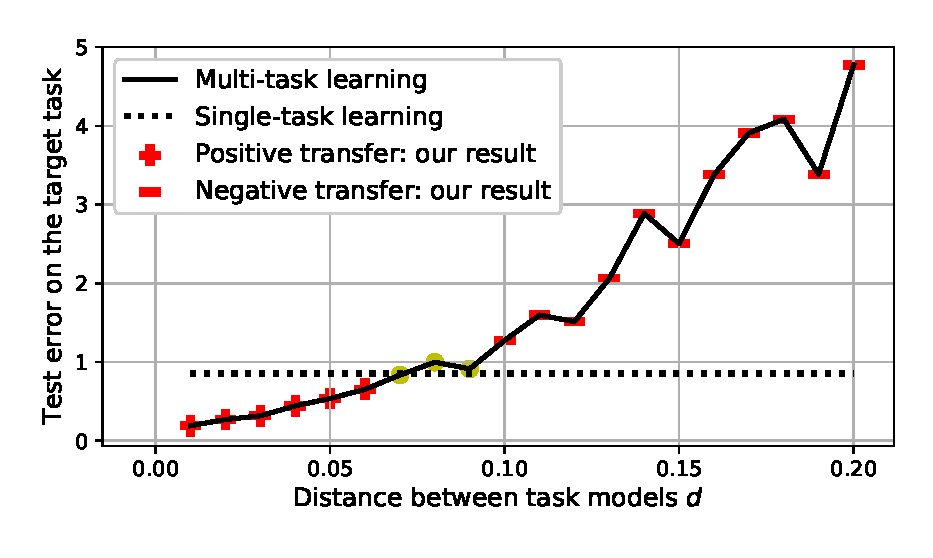
\includegraphics[width=0.5\textwidth]{figures/model_shift_phase_transition.eps}
	\caption{Positive vs negative transfer as a parameter of the task model distances.}
	\label{fig_model_shift_phasetrans}
\end{figure}


\subsection{Covariate Shift}

%\subsubsection{Gains over Single-Task Training}

Note that for the case of $k$ tasks with the same covariates, since there is no covariate shift and the data ratio is always equal to one, the main factor is model distance.

\paragraph{A precise bound when there is no model shift.}
As Proposition \ref{prop_monotone} shows, if $\beta_s$ and $\beta_t$ are equal, then adding the source task dataset always helps learn the target task.
The goal of this section is to understand how covariate shift affects the rate of transfer. \todo{add conceptual msg}

%The key quantity is to look at:
%The estimator using the source and target together from minimizing \eqref{eq_mtl_basic} is
%\[ \hat{\beta}_{s,t} = (X_1^{\top} X_1 + X_2^{\top} X_2)^{-1} (X_1^{\top}Y_1 + X_2^{\top}Y_2)\]
%The estimation error of $\hat{\beta}_{s,t}$ is
%\begin{align}\label{eq_two_task}
%  \err(\hat{\beta}_{s,t}) = \sigma^2 \cdot \tr[(X_1^{\top}X_1 + X_2^{\top} X_2)^{-1}].
%\end{align}
%The estimation error using the target alone is
%\begin{align}\label{eq_target_task}
%	\err(\hat{\beta}_t) = \sigma^2 \cdot \tr[(X_2^{\top} X_2)^{-1}].
%\end{align}
%The improvement of estimation error from adding the source task is then given by
%$\err(\hat{\beta}_t) - \err(\hat{\beta}_{s,t})$.
%For the test error on the target task, the improvement from adding the source task is
%\[ \te(\hat{\beta}_t) - \te(\hat{\beta}_{s,t}) = \sigma^2\cdot\bigtr{\bigbrace{(X_2^{\top}X_2)^{-1} - (X_1^{\top}X_1 + X_2^{\top}X_2)^{-1}}\cdot\Sigma_2}. \]

%We calculate the amount of improvement by comparing equation \eqref{eq_two_task} to equation \eqref{eq_target_task}.
A simple observation here is that when $\beta_s = \beta_t$, the optimal $\hat{w}$ for minimizing equation \eqref{eq_te_mtl} is equal to $1$.
Based on this observation, we can get a more precise result than Theorem \ref{thm_model_shift} on the improvement of adding the source task data that only depends on the covariance matrices $\Sigma_1, \Sigma_2$ and the number of data points $n_1, n_2$.

\begin{proposition}[Transfer rate without model shift]\label{thm_cov_shift}
	When $\beta_s = \beta_t$, we have that the optimal ratio for $W_1/W_2$ in equation \eqref{eq_te_mtl} satisfies
	$$1\le \hat{w} \le w_0:=1 +\frac{\sigma^2  \bigtr{(M^\top Z_1^{\top}Z_1 M)^{-1}} }{\left\|( M^\top Z_1^{\top}Z_1 M + Z_2^{\top}Z_2)^{-1} M^\top Z_1^{\top} Z_1 \Sigma_1^{1/2}\beta_t \right\|^2},$$%is $\hat{w} = 1 \pm \bigo{\frac 1 {n_1+n_2}}$ \todo{(figure out the constants)}
	where $M:=\Sigma_1^{1/2}\Sigma_2^{-1/2}$.
	And
	\begin{align*}
		%\err(\hat{\beta}^{\TL}_{s,t}) &= \sigma^2 \cdot \bigtr{\frac 1 {(n_1 + n_2)a_1\Sigma_1 + (n_1 + n_2)a_2\Sigma_2}} \\
		\te(\hat{\beta}^{\TL}_{t}) &= \sigma^2 \cdot \bigtr{\bigbrace{(n_1 + n_2)a_1\Sigma_2^{-1/2}\Sigma_1\Sigma_2^{-1/2} + (n_1 + n_2)a_2\id}^{-1}} + \bigo{|w_0-1|},
	\end{align*}
where $a_1, a_2$ are the solutions of equations \eqref{eq_a2}. \cor $w_0$ is close to 1 if the signal strength $\beta_t$ is much larger than the noise strength \nc
\end{proposition}


\begin{proof}
We abbreviate $\val(w_2\hat{B}(w)):=\val(w)$. We first notice that $\val (w) < \val (1)$ for all $0\le w < 1$. Thus we have $\hat w\ge 1$. It suffices to consider the case with $w> 1$. Under the assumption on $\beta_s$ and $\beta_t$, we can write
\begin{align}
	\val(w) =&~  \left( 1-\frac1w\right)^2 \left\|( M^\top Z_1^{\top}Z_1 M + w^{-2}Z_2^{\top}Z_2)^{-1} M^\top Z_1^{\top} Z_1 \Sigma_1^{1/2}\beta_t \right\|^2 \nonumber \\
			&~ + \frac{\sigma^2}{w^2} \cdot \bigtr{( M^\top Z_1^{\top}Z_1 M + w^{-2}Z_2^{\top}Z_2)^{-1} }. \nonumber
\end{align}
Since
$$\left\|( M^\top Z_1^{\top}Z_1 M + w^{-2}Z_2^{\top}Z_2)^{-1} M^\top Z_1^{\top} Z_1 \Sigma_1^{1/2}\beta_t \right\|^2 = \tr \left[ ( M^\top Z_1^{\top}Z_1 M + w^{-2}Z_2^{\top}Z_2)^{-2}M^\top Z_1^{\top} Z_1 \Sigma_1^{1/2}\beta_t\beta_t^\top \Sigma_1^{1/2}Z_1^{\top} Z_1  M\right]$$
is increasing with respect to $w$, then the derivative of $\val(w)$ can be bounded from below as
\begin{align*}
\val'(w) \ge &~ 2\frac{w-1}{w^3} \left\|( M^\top Z_1^{\top}Z_1 M + w^{-2}Z_2^{\top}Z_2)^{-1} M^\top Z_1^{\top} Z_1 \Sigma_1^{1/2}\beta_t \right\|^2   \\
			&~ - 2 \frac{\sigma^2}{w^3} \cdot \bigtr{(M^\top Z_1^{\top}Z_1 M +w^{-2}  Z_2^{\top}Z_2)^{-1} M^\top Z_1^{\top}Z_1 M (M^\top Z_1^{\top}Z_1 M + w^{-2} Z_2^{\top}Z_2)^{-1}} \\
\ge &~ 2\frac{w-1}{w^3} \left\|( M^\top Z_1^{\top}Z_1 M +  Z_2^{\top}Z_2)^{-1} M^\top Z_1^{\top} Z_1 \Sigma_1^{1/2}\beta_t \right\|^2   - 2 \frac{\sigma^2}{w^3} \cdot \bigtr{(M^\top Z_1^{\top}Z_1 M)^{-1}}.
			%\\ =& ~ 2\frac{d^2}{w^3} \tr\left[( M^\top Z_1^{\top}Z_1 M + w^{-2}Z_2^{\top}Z_2)^{-1} M^\top Z_1^{\top} \left[\left( w-1\right)\left(Z_1 \Sigma_1 Z_1^{\top}\right) - \frac{\sigma^2}{d^2}\id \right] Z_1 M ( M^\top Z_1^{\top}Z_1 M + w^{-2}Z_2^{\top}Z_2)^{-1}\right]  .
\end{align*}
Hence $\val'(w)\ge 0$ if $w\ge w_0$, i.e. $\val(w)$ is an increasing function on $[1+w_0,\infty]$. Thus we get $\hat w$ is between $[1,w_0]$.
\end{proof}



As a remark, we see that Proposition \ref{prop_monotone} follows from Theorem \ref{thm_cov_shift}.
The amount of reduction on test error for the target task is given as
	\begin{align*}
%		\err(\hat{\beta}_t) - \err(\hat{\beta}_{s,t})
%		&= \sigma^2 p \cdot \bigtr{\frac 1 {(n_2 - p) \Sigma_2} - \frac 1 {(n_1 + n_2)a_1 \Sigma_1 + (n_1 + n_2)a_2 \Sigma_2}}, \\
		\te(\hat{\beta}_t) - \te(\hat{\beta}_{s,t})
		&= \sigma^2 \cdot \bigbrace{\frac p {n_2 - p} -  \bigtr{\bigbrace{(n_1 + n_2)a_1\Sigma_2^{-1/2}\Sigma_1\Sigma_2^{-1/2} + (n_1 + n_2)a_2\id}^{-1}}}.
	\end{align*}
Because
\begin{align*}
	\te(\hat{\beta}_{s,t}) \le \te(\hat{\beta}_t)
	\Leftarrow~ & (n_2 - p)\Sigma_2 \preceq (n_1 + n_2) a_1 \Sigma_1 + (n_1 + n_2)a_2 \Sigma_2 \\
	\Leftrightarrow~ & \zeroMatrix \preceq (n_1 + n_2) a_1 \Sigma_1 + (n_1 - (n_1 + n_2)\cdot a_1) \Sigma_2,
\end{align*}
which is true since $a_1 \le n_1 / (n_1 + n_2)$ by equation \eqref{eq_a2}.
The proof for $\te(\hat{\beta}_{s,t}) \le \te(\hat{\beta}_t)$ follows by multiplying $\Sigma_2^{-1/2}$ on both sides of the inequalities above.

\medskip
Now we apply Theorem \ref{thm_cov_shift} to show how covariate shift affects the rate of transfer.

%\begin{example}[\textbf{When $\Sigma_1 = \Sigma_2$}]
%In this case, we have $\lambda_i = 1$ for all $1\le i\le p$.
%And $a_1 + a_2 = 1 - p / (n_1 + n_2)$.
%Hence
%\[ \te(\hat{\beta}_{s,t}) = \frac{\sigma^2 p^2}{n_1 + n_2 - p} \text{ and } \err(\hat{\beta}_{s,t}) = \frac {\sigma^2 p} {n_1 + n_2 - p} \bigtr{\Sigma_2^{-1}}. \]
%\end{example}

\smallskip
\begin{example}[\textbf{When $\Sigma_1 = \Sigma_2 / \lambda$}]
In this case, equations \eqref{eq_a2} become
\[ a_1 + a_2 = 1 - p/(n_1 + n_2), a_1 + \frac{p}{n_1 + n_2} \cdot \frac {a_1} {a_1 + \lambda^2 a_2} = \frac{n_1} {n_1 + n_2}. \]
By solving these, we can get the test errors (the estimation error behaves similarly).
Figure \ref{fig_te_scaling} shows how they grow as we increase the number of source task data points.
Here $n_2 = 4p$ and $n_1$ ranges from $p$ to $20p$.
We can see that the smaller $\lambda$ is, the lower the test errors will be.
\end{example}

\smallskip
\begin{example}[\textbf{When $\Sigma_1$ and $\Sigma_2$ are complementary}]\label{example comple}
	We now consider another case when $\Sigma_1$ and $\Sigma_2$ have complementary eigenspaces. Suppose $\Sigma_1$ and $\Sigma_2$ have the eigendecomposition
$$\Sigma_1^{1/2} = 1+ U\Lambda U^\top, \quad \Sigma_2^{1/2} = 1+ V\Lambda V,$$
where
$$\Lambda = \diag(\wt\lambda_1,\cdots, \wt\lambda_{p/2}), \quad U= (u_1,\cdots, u_{p/2}), \quad V= (v_1,\cdots, v_{p/2}).$$
If $V=U_\perp$, i.e. the vectors $v_1,\cdots, v_{p/2}$ are perpendicular to the vectors $u_1,\cdots, u_{p/2}$, then
$$M=\Sigma_1^{1/2} \Sigma_2^{-1/2}=(1+\Lambda)UU^\top + (1+\Lambda)^{-1}V V^\top .$$

As a concrete example we consider the case where $\wt \lambda_1=\cdots=\wt\lambda_{p/2}$ and we denote $\lambda:=1+\wt\lambda_1$. Thus for $M$, the first $p/2$ singular values are equal to $\lambda$ and the rest ones are equal to $\lambda^{-1}$. In this case, equations in \eqref{eq_a2} become
\be\label{compleeq} a_1 + a_2 = 1 - \frac{p}{n_1 + n_2},  \ \ a_1 + \frac{p}{2(n_1 + n_2)}\cdot \bigbrace{\frac{a_1}{a_1 + \lambda^2 a_2} + \frac{a_1}{a_1 + \frac{a_2}{\lambda^2}}} = \frac{n_1}{n_1 + n_2}. \ee
It's not hard to verify that there is only one valid solution $(a_1,a_2)$ to \eqref{compleeq}. After solving these, we get the test error for the target task as follows.
\be\label{testcomple}
te(\lambda)=\frac{p}{2(n_1 + n_2)} \cdot \bigbrace{\frac{1}{\frac{a_1}{\lambda^2} + a_2} + \frac{1}{a_1\lambda^2 + a_2}}.\ee

In Figure \ref{fig_te_complement}, we plot the test error of the target task for $n_2 = 4p$ and $n_1$ ranging from $p$ to $20p$. First we notice that the curves in Figure \ref{fig_te_complement} all cross at the point $n_1=n_2$. In fact, if $n_1=n_2$, then it is easy to observe that $a_1=a_2=(1-\gamma)/2$ is the solution to equation \eqref{compleeq}, where we denote $ \gamma=p/(n_1+n_2)$. Then for any $\lambda$, the test error in \eqref{testcomple} takes the value
$$te(\lambda)= \frac{\gamma}{2}\frac{1}{(1-\gamma)/2}=\frac{p}{n_1+n_2-p}.$$

Second, we observe the following two phases as we increase $n_1 / p$.
\begin{itemize}
	\item When $n_1 \le n_2$, having complementary covariance matrices leads to lower test error compared to the case when $\Sigma_1 = \Sigma_2$.
	\item When $n_1 > n_2$, having complementary covariance matrices leads to higher test error compared to the case when $\Sigma_1 = \Sigma_2$.
\end{itemize}
%Second, from Figure \ref{fig_te_complement} we observe that the complementary cases with $\lambda>1$ is better than the case without covariate shift (i.e. $M=\id$ case) when $n_1<n_2$. On the other hand, if we have enough source task data such that $n_1>n_2$, then it is always better to have no covariate shift.
This phenomenon can be also explained using our theory. With \eqref{compleeq}, we can write
$$te(\lambda)=\frac{\gamma}{2} \cdot \bigbrace{\frac{1}{\frac{a_1}{\lambda^2} + (1-\gamma - a_1)} + \frac{1}{a_1\lambda^2 + (1-\gamma - a_1)}}.$$
We can compute that
\begin{align*}
te(\lambda) - te(1)&= \frac{\gamma}{2(1-\gamma)} (\lambda^2-1)a_1\cdot \bigbrace{  \frac{1}{ -a_1(\lambda^2-1)+(1-\gamma)\lambda^2 } - \frac{1}{a_1(\lambda^2-1) + (1-\gamma)}} \\
&= \frac{\gamma}{2(1-\gamma)} (\lambda^2-1)^2 a_1\cdot  \frac{2a_1 - (1-\gamma) }{[-a_1(\lambda^2-1)+(1-\gamma)\lambda^2 ][a_1(\lambda^2-1) + (1-\gamma)]} .
\end{align*}
If $n_1>n_2$, we have $a_1>(1-\gamma)/2$ (because $a_1>a_2$ as observed from the equation \eqref{compleeq}), and hence $te(\lambda)>te(1)$. Otherwise if $n_1< n_2$, we have $a_1< (1-\gamma)/2$, and hence $te(\lambda)< te(1)$.

\end{example}

We can extend the above observation for Example \ref{example comple} to more general cases with arbitrary covariate shift. To compare different choices of $M$, we need to fix a scaling for them, because otherwise $aM$ always achieves a smaller error than $M$ for $a>1$. For this purpose, we introduce the following condition
\be\label{GMcons}\det(M^\top M)= a^p \Leftrightarrow \prod_{i=1}^p \lambda_i = a^p\ee
for some constant $a>0$, and compare different choices of $M$ under this constraint. The next proposition shows that, roughly speaking, as long as there are sufficiently many source task datas, then $M=a\id$ always gives (approximately) the smallest test error.
\begin{proposition}
We have that the test error satisfies
\be\label{approxteM}  te(M)\left(1 -  \frac{n_2}{n_1-p} \frac{1}{\lambda_p^2 + \frac{n_2}{n_1-p}}\right)  \le  \frac{\sigma^2}{n_1+n_2}\tr\left( \frac{1}{a_1M^\top M + a_2}\right) \le te(M),\ee
where $\lambda_p$ is the smallest singular value of $p$ and
$$te(M):= \frac{\sigma^2}{a_1(n_1+n_2)}\tr\left( \frac{1}{M^\top M}\right) .$$
Moreover, for all $M$ satisfying \eqref{GMcons}, the minimum of $te(M)$ is attained when $M= a\id$.
\end{proposition}
\begin{proof}
From equation \eqref{eq_a2}, we get
$$a_1\ge \frac{n_1-p}{n_1+n_2},\quad a_2\le \frac{n_2}{n_1+n_2}.$$
With these two bounds, we can easily conclude \eqref{approxteM}.

For the second statement, we find that we need to minimize
$$\tr\left( \frac{1}{M^\top M}\right) = \sum_{i=1}^p\frac{1}{\lambda_i},\quad \text{under}\ \ \prod_{i=1}^p\lambda_i=a^p.$$
Then using AM-GM inequality, we conclude that the sum $\sum_{i=1}^p\lambda_i^{-1}$ is smallest when $\lambda_1=\cdots=\lambda_p = a$.
\end{proof}

From the above proposition, we see that when $n_1\gg n_2$, we have that the test error is approximately given by $te(M)$ (as long as we impose a proper lower bound on $\lambda_p$). Moreover, $te(M)$ is minimized when $\Sigma_1$ and $\Sigma_2$ are proportional to each other, i.e. there is no covariate shift between the source task data and target task data. This provides a theoretical evidence that in general covariate shift is unfavored in transfer learning if we have enough source task data, although Example \ref{example comple} show that this may not be true when the number of source task data is small.

%then the choice $M^\top M = a^{1/p}\id $ achieves the smallest test error. In fact, for sufficiently large $n_1$, we have $a_1\approx 1-\gamma$ and $a_2\approx 0$.




\begin{figure}
	\centering
	\begin{minipage}{0.48\textwidth}
		\centering
		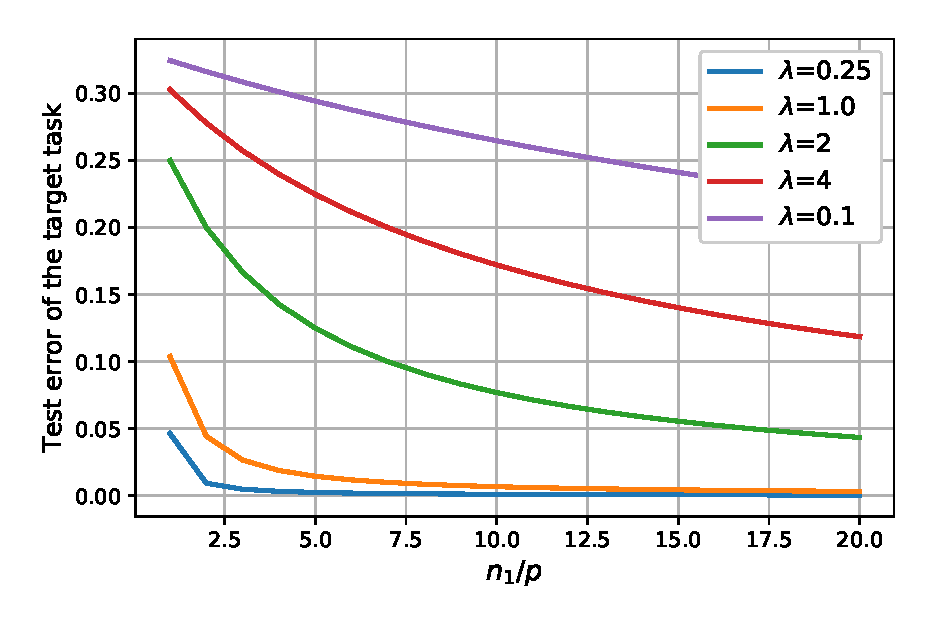
\includegraphics[width=0.9\textwidth]{figures/scaling.eps}
		\caption{When $\Sigma_1 = \Sigma_2 / \lambda$.}
		\label{fig_te_scaling}
	\end{minipage}\hfill
	\begin{minipage}{0.48\textwidth}
		\centering
		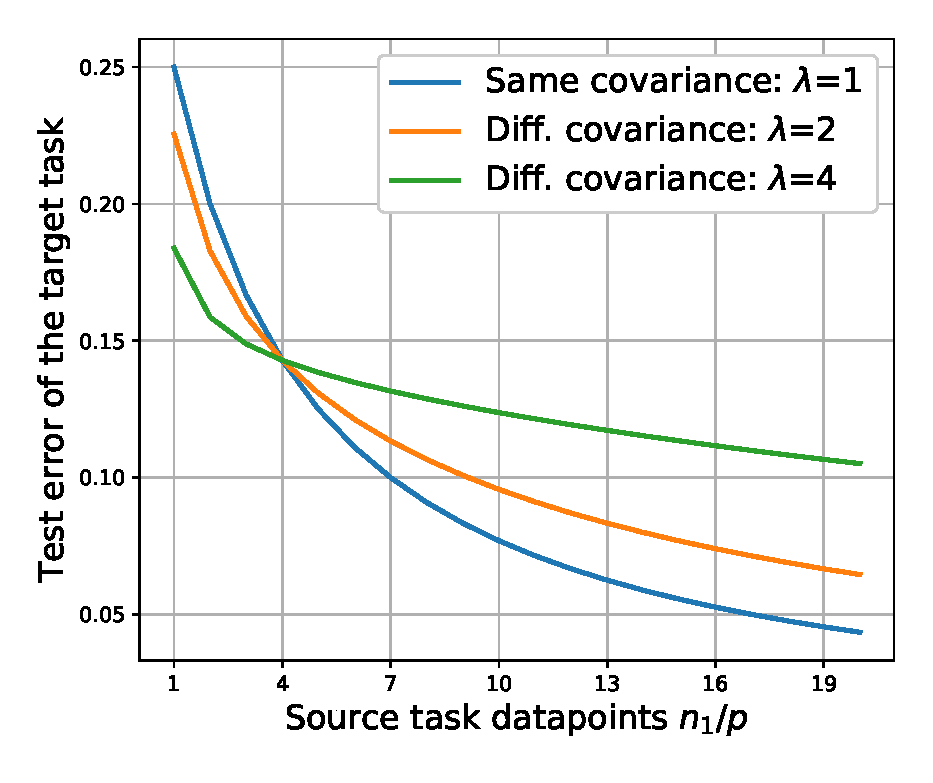
\includegraphics[width=0.9\textwidth]{figures/complementary.eps}
		\caption{When $\Sigma_1$ and $\Sigma_2$ are complementary. The number of target task data points is $n_2 = 4p$.}
		\label{fig_te_complement}
	\end{minipage}
\end{figure}


\paragraph{Extending the intuition to the general case.}
When there is model shift, i.e. $\beta_s = \beta_t$, we can still use Theorem \ref{thm_model_shift} (and Proposition \ref{prop_model_shift_tight}) to get the result.
\begin{itemize}
	\item \textbf{The effect of covariate shift:}
	\item \textbf{The effect of data ratio:}
\end{itemize}

\subsection{Data Ratio}